% This is samplepaper.tex, a sample chapter demonstrating the
% LLNCS macro package for Springer Computer Science proceedings;
% Version 2.20 of 2017/10/04
%
\documentclass[runningheads]{llncs}
%

\usepackage{multirow}
\usepackage{cite}
\usepackage{tabularx}
\usepackage{booktabs}
\usepackage{caption}
\usepackage{geometry}
\usepackage{graphicx}

\usepackage[hyphens]{url}
\usepackage{hyperref}
\hypersetup{breaklinks=true}
\hypersetup{
    colorlinks=false,
    pdfborder={0 0 0},
}

\urlstyle{same}
\usepackage{cite}
% Used for displaying a sample figure. If possible, figure files should
% be included in EPS format.
%
% If you use the hyperref package, please uncomment the following line
% to display URLs in blue roman font according to Springer's eBook style:
% \renewcommand\UrlFont{\color{blue}\rmfamily}

\begin{document}
%
\title{Brain Age Prediction using Topological Graph Augmentation and Graph Neural Networks}



\author{ Ufuk Cem Birbiri}
\institute{
Université Côte d'Azur \\
\email{ufuk-cem.birbiri@etu.univ-cotedazur.fr}
}
 








\maketitle              % typeset the header of the contribution
%
\begin{abstract}



Many common neurological and neurodegenerative disorders, such as Alzheimer’s disease, Parkinson's disease, or autism have been linked with anomalous patterns of biological aging of
the brain. Discovering which brain regions are related to specific neurological disorders or cognitive stimuli became an essential field of neuroimaging research. Diffusion Tensor Images (DTI) can be used to reveal the biological underlying patterns behind the aging process, holds an individual's signs for various brain disorders, and
propose new personalized-treatment approaches. In this work, we used the brain network graph representations of 998 patients. The nodes represent the brain regions and the edges are described as interactions between the regions. We trained a Graph Neural Network to predict four brain age classes [$22$-$25$, $26$-$30$, $31$-$35$, $36+$]. To increase the accuracy of the model we propose a topological graph data augmentation method. We used the Mapper algorithm to convert brain graphs into the topological complex where each feature of the complex represents brain activations between regions. Based on our quantitative results, the GNN gained a 0.64 test accuracy using only raw graphs, and 0.776 test accuracy using both raw graphs and topological augmented graphs. Using topological graph representations of the brain helped to reveal the functional connectivity of the brain and increased the model performance.




\keywords{Brain age  \and Graph Neural Network \and Topological complex}
\end{abstract}
%
%
%
\section{Introduction and Related Work}

The relation between the neurological and neurodegenerative disorders and deviational brain aging pathways has inspired a great number of research topics
in brain age prediction using neuroimaging data\cite{kaufmann2019common, bonacich1987power, franke2019ten}. The estimations of brain age gaps, described as
the difference between the estimated brain age and the true
biological age, have been related to brain diseases such as dementia and autism, Alzheimer's disease, Parkinson's, or Epilepsy\cite{nalls2013multicenter, tuncc2019early}, and therefore could be beneficial in monitoring and treatment of disease.

Various studies used machine learning in brain age prediction, mostly using genetic information and magnetic resonance imaging(MRI)\cite{franke2019ten}. These studies mostly
do not include other brain imaging modalities such as time-series data
of functional MRI(fMRI), clinical test results, or the expertise
of psychiatrists, or neuroscientists. Still, different modalities show improvement in the results\cite{kaufmann2019common, besteher2019machine, baecker2021machine}.

To estimate brain age in a clinically applied fashion, we used Graph Neural networks(GNN). GNN
provides a deeper way of learning of brain mapped as a graph structure and it is rapidly becoming the state-of-the-art approach in various network neuroscience problems. The brain is an exceptionally complex system and understanding its functional organization is the goal of understanding various diseases. The motivation behind brain age estimation is to have a GNN network to predict human age by using the brain regions as nodes whose features will reveal brain activation in such patients. 

Here we used Diffusion Tensor Images (DTI) of patients represented as a connectivity matrix of the brain. The connectivity matrix has been converted to a graph where the nodes in the graph are characterized as brain regions and edges as the functional connectivity between brain regions, computed as the pairwise interactions
of DTI.  We analyzed the effectiveness of GNN for brain
age prediction by training Graph Convolutional Network\cite{berg2017graph} between four age groups. We additionally investigate adding topological graph representation of the brain networks as a data augmentation method to increase prediction accuracy. 





\section{Methods}
In this section, we describe the dataset and the task description as well as the topological data augmentation method applied to brain networks.



\subsection{Dataset}
The data includes 998 patients belonging to Human Connectome Project (HCP)~\cite{dataset_info1}. Each patient has a DTI scan represented as brain network activation during a period. The brain networks consist of brain regions and their interactions with each other. Each patient has a brain network scan represented as a connectivity matrix in which rows and columns are described as brain regions, the values represent the interactions between two regions. Connectivity matrices measure the number of fibers from one region to another region of the brain. 

In addition, there are other clinical variables for the 998 patients in the dataset such as age, gender, diseases, past injuries, disease history, brain regions' volume, surface area, thickness, grey matter volume as well as cognitive test scores, motor skills, sensory, and emotion. The dataset includes very different clinical information for each patient. If we understand their brain network functioning, we could be able to understand specific cases for example an Alzheimer patient's brain functioning. Age prediction is important since age is the most effective and relatable parameter in such diseases\cite{kaufmann2019common}. Building a Graph network that can predict a patient's age correctly will contribute to disease analysis in neurological research.

\subsection{Task Description}
In this work, we represented the brain networks as connectivity matrices shape (116, 116) meaning that rows and columns are 116 brain regions. There is one matrix for each patient and each represents a weighted undirected graph. The elements of the matrix are the number of fibers in between the regions after normalization. The connectivity matrices are converted to undirect graphs using the Networkx library\cite{Networkx} where nodes represent the 116 regions, and edges represent interactions. Figure \ref{fig1} shows an example of a connectivity matrices of a patient with its graph visualization. The different brain regions are shown in the matrice such as $Precentral\_L$	as the left Precentral gyrus, $Frontal\_Sup\_L$ as the left Superior frontal gyrus-dorsolateral, and 
$Frontal\_Sup\_Orb\_L$	as left Superior frontal gyrus-orbital.

%
\begin{figure}[!h]
  \centering
  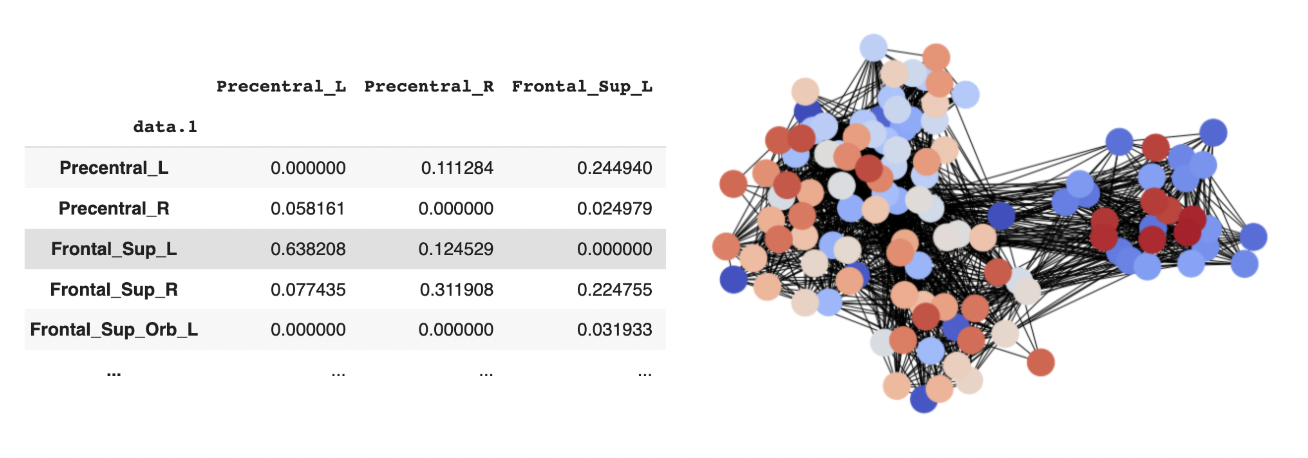
\includegraphics[width=12cm]{images/Fig1.png}
  \caption{\textit{((Left) An example of a brain connectivity matrix of size $116\times 116$ that belongs to a male patient with age $36+$. The rows and columns represent brain regions. (Right) The graph visualization of the same patient's connectivity matrix where nodes represent brain regions.}}
  \label{fig1}
\end{figure}
%
The patient's age differs from four categories [$22$-$25$, $26$-$30$, $31$-$35$, $36+$] and the class ratio of the ages in the dataset are 17\%, 35\%, 25\%, and 23\%, respectively. The problem, therefore, turns into a multi-class graph classification problem with four different classes. 
\subsection{Dataset Preparetion}
GNNs for graph classification have been used in network neuroscience\cite{bessadok2022graph}, drug discovery to classify molecules as toxic or non-toxic~\cite{wieder2020compact}, or in text classification~\cite{huang2019text}. To use our dataset in the GNN network we need to use the \emph{torch.geometric Data} type. 
In our task, each brain network is represented as a graph with node and edge features. The edge attributes are assigned as interaction values and the node features are assigned as the eigenvector centrality of the nodes.\\

\textbf{Eigenvector Centrality}\\
 The eigenvector centrality for node 
$i$ is the $i$\textsuperscript{th} entry of the vector characterized by the equation
 \[ Ax = \lambda x, \]
where 
$A$ is the adjacency matrix of the graph $G$ with eigenvalue $\lambda$. By the Perron–Frobenius theorem~\cite{bonacich1987power}, one can conclude that there exists a unique solution 
$x$. If $\lambda$ is the largest eigenvalue of the adjacency matrix $A$, we can say that the unique solution $x$ has positive values in all of the entries~\cite{brede2012networks}. As a result, the eigenvector centrality of each of the nodes is calculated $G$ and assigned as the node attribute. 

  \subsection{Graph Convolutional Network}
The GNN model was adopted from the `Semi-supervised Classification with Graph Convolutional Networks'~\cite{kipf2016} that uses the graph convolutional operator. In this network, three graph convolutional layers (GCNConv~\cite{GCNConv}) were used followed by a linear layer. The Relu activation function is added as an activation function. To overcome the over-fitting, dropout is used before the last linear layer. In addition, Pytorch geometric provides a pooling layer called $global$\_$mean$\_$pool$ located before the dropout which returns batch-wise and graph-level outputs by taking the average of node features across the node dimensions\cite{Poolinglayers}. The GNN model is shown in the Appendix section.\\
To increase the number of graphs in the dataset and represent the brain networks in a better way, we propose the topological graph augmentation method.

%
\begin{figure}[!ht]
  \centering
  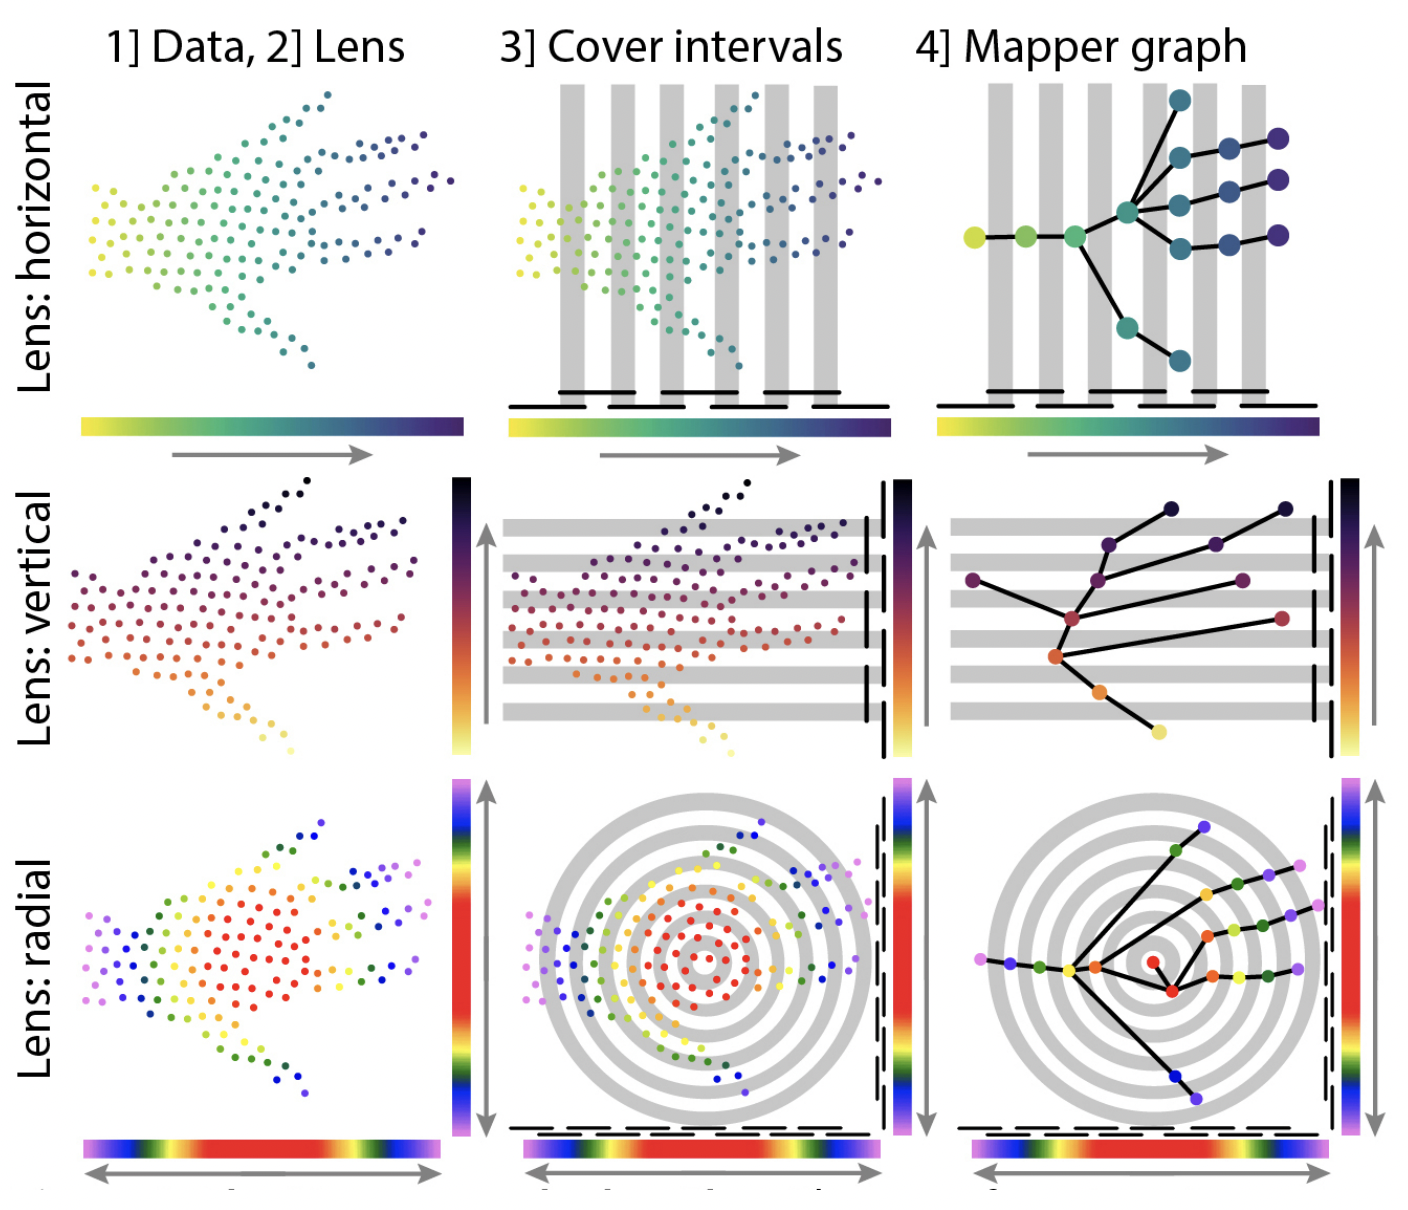
\includegraphics[width=12cm]{images/different_filters.png}
  \caption{\textit{Three different lenses(filters) on the same point cloud data. The rows show the horizontal, vertical, and radial filter selection results, respectively. The data, the cover intervals(gain and resolution parameters), and the Mapper result are shown in the left, middle, and right columns respectively. The image is taken from~\cite{chazal2021introduction}.}}
  \label{different_filters}
\end{figure}
%

\subsection{Data Augmentation Using Topological Complex}
Understanding the \textit{shape of data} brings us to topology, which is a branch of mathematics. Over the last 20 years, topological techniques have been used in various applied problems, one of these fields is called Topological Data Analysis (TDA). TDA provides detailed information about the characteristics of the data by providing some topological, statistical, and geometrical methods to infer complex topological structures such as connected components, holes, branches, or loops. This analysis method is very robust to outliers and noise where the data is usually represented as point clouds or distance matrices in a Euclidean metric space.

Each brain network graph is converted to a topological complex called the Mapper complex using the GUDHI Python library\cite{gudhi}. Mapper is a computational method for complex datasets to extract the simplest information in the form of $simplicial-complexes$ that preserve the underlying topological structures from the original data. It uses metrics and lenses to convert data into a topological network where nodes represent similar data points and edges represent topological relations. The key idea of the Mapper algorithm is to map data points into a metric space using some filters defined on data points while capturing topological and geometric information at a specified resolution and gain. The filter function (also called a lens) is the metric that allows us to map our data points. The choice of the filter is an important factor for achieving a good result in the Mapper. The results of different filter functions are shown in Figure \ref{different_filters}. In the figure, three different filters (horizontal, vertical, and radial) are applied to the same data. It can be seen that different filter functions have different results.  Therefore, selecting the filter functions for the Mapper algorithm plays a critical role.

The most commonly used filters are Singular Value Decomposition (SVD) and L-Infinity centrality based on their quantitative performances in topological data analysis\cite{nielson2015topological, lum2013extracting, banerjee2017microbial}. The two filter functions are also selected as L-Infinity and SVD as the first and second filters, respectively. L-infinity centrality assigns a value to each data point which is the furthest distance from itself to another data point. Basically, for each data point y, it amounts to finding the maximum distance from y to any other point in the dataset. Large values of this filter put points that are far away from the center of the dataset. On the other hand, SVD is a linear dimension reduction technique that does not center the data points before the actual computation, meaning that it efficiently works with sparse data. We used the first component of the SVD in the Scikit-learn library\cite{SVD}

The other parameters in the Mapper are the resolution and the gain. Resolution is the number of intervals required to cover each filtered image. If the resolution is increased, then the number of communities in the resulting graph will also increase. The communities refer to the nodes clustered together in the Mapper. This parameter is tested in the range [2-50] and selected as 20. The gain parameter is the percentage of overlaps between the intervals covering each filtered image. It should be between 0 and 1 and selected as 0.25. In addition, the clustering algorithm is selected as $DBSCAN$. Parameter selection was done based on a literature search and we choose the parameters that give the highest accuracy in the GNN model. 

%
\begin{figure}[!ht]
  \centering
  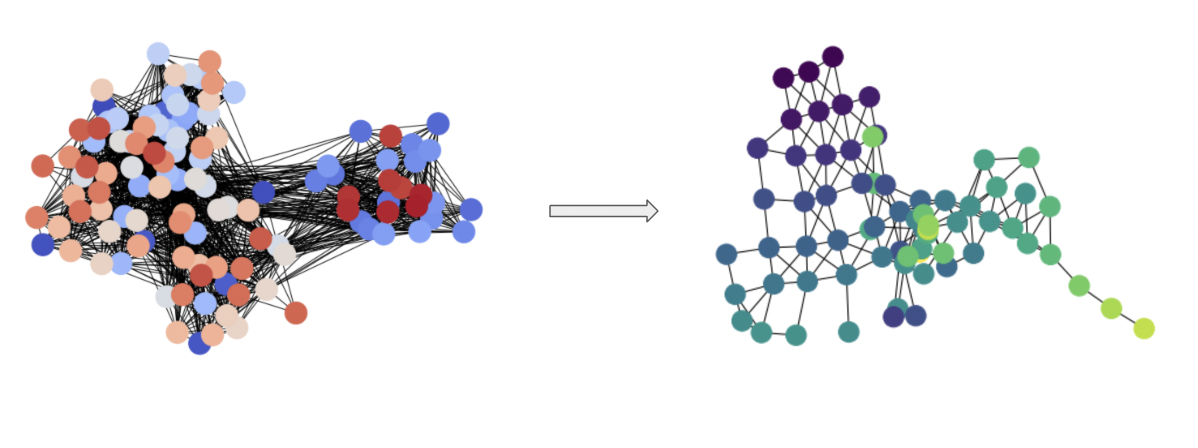
\includegraphics[width=12cm]{images/after_mapper.png}
  \caption{\textit{(Left) The brain network is displayed as a Networkx graph. (Right) The result of the Mapper algorithm. }}
  \label{after_mapper}
\end{figure}
%

The Mapper algorithm is applied for each brain network graph and achieved a Mapper complex representation of the graphs. The Mapper complex is another Networkx graph with fewer nodes as edges since similar brain activations clustered together during the complex computation. The result of the same patient after the Mapper is shown in Figure \ref{after_mapper}. The nodes in the Mapper complex represent clustered brain regions and edges represent high-order interactions of the brain regions. The colors in both graphs do not mean anything and are used only for visualization. More Mapper results can be found in the Appendix section.


\subsection{Training}
 Two different datasets were created for the GNN model. The first one consists of only 998 raw brain network graphs. The second dataset contains both raw brain network graphs(998) and topological graphs(998) resulting in 1996 graphs in total. The dataset was split into training(70\%) and testing(30\%). To obtain objective results, the test set included only raw graphs, and the testing data was only used in the testing phase. To achieve a better validation of the experiments, 4-fold cross-validation was performed. The models were trained
with 150 epochs with a learning rate = 0.0005 using the cross-entropy loss function.


\section{Results}

The task is the multi-class graph classification with four different age groups in terms of [$22$-$25$, $26$-$30$, $31$-$35$, $36+$]. It is a so-called balanced dataset that represents mostly the younger and mature phases of humans. The performance of the Graph Convolutional Network will be tested on both the $raw$ graph dataset and the $raw+topological$ graph dataset. The accuracy results are shown in Table~\ref{tab:my_label}.



\begin{table}
    \centering
    \caption{The training and testing accuracy results of multi-class classification of the network.}
    \label{tab:my_label}
    \begin{tabularx}{12cm}{XXX}
    \toprule
    \textbf{Training datasets } & \textbf{Train accuracy} & \textbf{Test accuracy }\\
    \midrule
    Raw graphs & 0.634 $\pm$ 0.15  &\textbf{ 0.640 $\pm$ 0.32 }\\ 

    Raw + Topological graphs & 0.782 $\pm$ 0.12 &\textbf{ 0.776 $\pm$ 0.20 }\\ 
    \bottomrule
    \end{tabularx}
\end{table}


When we use only the raw brain graphs we achieve 0.634 training and 0.640 test accuracy. If we add the topological complex representations of the brain networks the age prediction accuracy achieved 0.782 in the training set and 0.776 in the testing set. The topological data augmentation not only increased the number of graphs in the dataset but also gave a chance to GNN to learn better from topological brain networks. The Mapper complex is the topological structure of the brain networks and its topological features represent brain activation. A topological feature can be a connected component, a 1D hole/loop, a 2D cavity, or more generally a d-dimensional “void” which preserves the interactions between different brain regions. 

The proposed model could be used for the prediction of age in humans. The proposed graph representations capture informative features of the brain by linking the interaction among different brain regions.

\section{Conclusion}
The human brain is an enormously complex system and discovering its functional connectivity is the goal of neuroscience research. Many diseases can be related to brain age such as Epilepsy, stroke, Amyotrophic Lateral Sclerosis (ALS), or trauma. Understanding aging and its effects on various disorders can reveal much information about brain functioning. Diffusion Tensor Imaging is a novel imaging method that can reveal unique information about white matter within the brain regions. In this work, we presented brain networks of 998 patients as graphs created from DTI connectivity matrices. We used a Graph Convolutional Network to predict the brain age of patients in four different age categories. Also, we propose topological graph augmentation methods to analyze brain activation using the Mapper complex. The proposed method increased the GNN performance.


\section{Perspectives}
For the future of this study, we can different directions to understand complex brain structure and functioning. Each sample in the dataset was a DTI scan of a patient and it is represented by a graph. Significantly, the nodes are described as brain regions and edges are the functional connectivity between them. The Graph Convolution layers can be analyzed with some feature engineering to understand which brain regions(nodes) were more effective for age prediction. Can we relate these regions with the patient's specific disease(Alzheimer, autism, etc)? Do these regions have anomalies in brain thickness, surface area, or (less) gray matter volume?
We also used Topological data augmentation where we convert the brain network graphs into a topological complex called the Mapper complex. In the Mapper complex, the nodes were mapped by two filter functions and followed by clustering. Which brain regions are clustered and why? How to improve the classification accuracy by using different filters in Mapper. The subgroup analysis on brain regions to understand the interaction between brain regions~\cite{vallartatopological, nicolau2011topology}.
\section{Acknowledgements}

This project is a part of the M2 studies and has collaboration with \textit{the Inria Center at Universit{\'e} C{\^o}te d'Azur, Sophia Antipolis, France} under the supervision of \textit{Mathieu Desroches}, and \textit{the University of Amsterdam} under the supervision of \textit{Fernando a. Nóbrega Santos}. We would like to thank \textit{Serafim Rodrigues} from \textit{BCAM - Basque Center of Applied Mathematics} for his valuable discussions and support throughout the project. His ideas and expertise were instrumental in shaping the direction of this research.


% the environments 'definition', 'lemma', 'proposition', 'corollary',
% 'remark', and 'example' are defined in the LLNCS documentclass as well.
%

%
% ---- Bibliography ----
%
% BibTeX users should specify bibliography style 'splncs04'.
% References will then be sorted and formatted in the correct style.
%
% \bibliographystyle{splncs04}
% \bibliography{mybibliography}
%


\bibliographystyle{myunsrt}
\small
\bibliography{rapport}

\newpage

\section*{Appendix}
In this section, we will demonstrate some visualizations of the Mapper complex. In Figure~\ref{appendix}, four different patients' brain maps before and after the Mapper complex computation on the left and right columns, respectively. The age of the patients belongs to the following ranges respectively: [$22$-$25$, $26$-$30$, $31$-$35$, $36+$].
%
\begin{figure}[!ht]
  \centering
  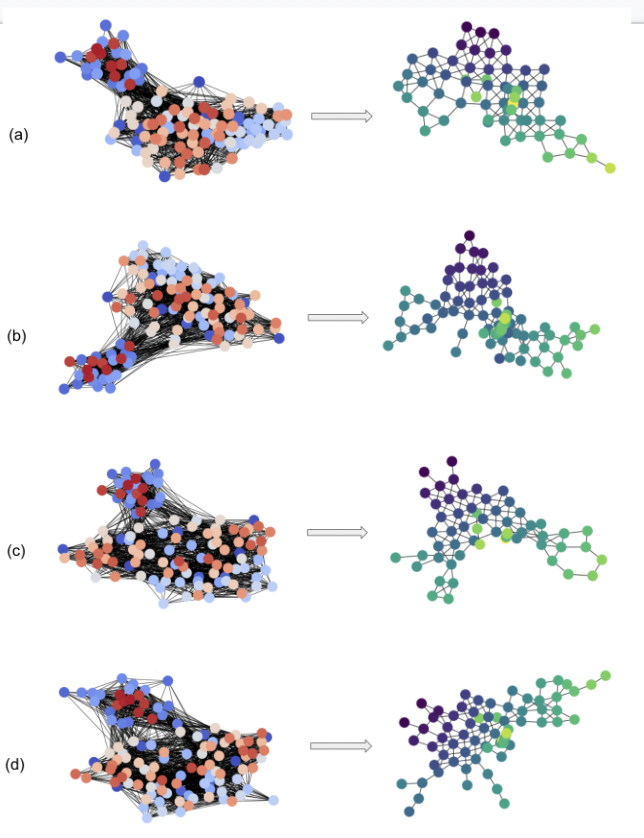
\includegraphics[width=10cm]{images/Appendix.png}
  \caption{\textit{ }}
  \label{appendix}
\end{figure}
%

In Figure~\ref{GNN_model}, the Graph Convolutional model that is used in this work is shown. There are three convolutional layers followed by a dropout and a linear layer. 

%
\begin{figure}[!ht]
  \centering
  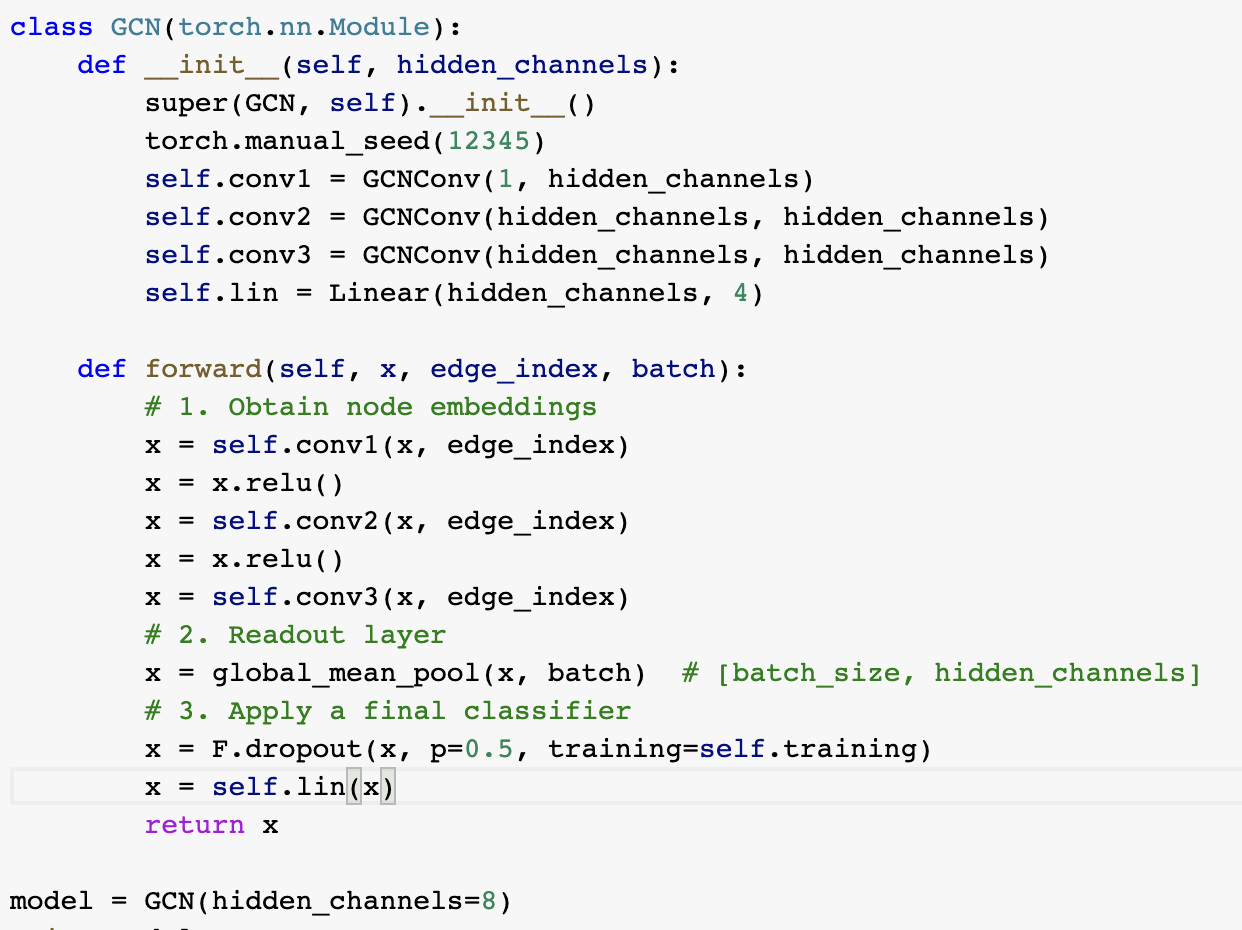
\includegraphics[width=11cm]{images/GNN_model.png}
  \caption{\textit{The GCN model for the graph classification task.}}
  \label{GNN_model}
\end{figure}
%

\end{document}
